
%%%%%%%%%%%%%%%%%%%%%%%%%%%%%%%%%%%%%%%%%%%%%%%%%%%%%%%%%%%%%%%%%%
\chapter{Hydrogen atom - polynmomial method}
\label{atom}
%%%%%%%%%%%%%%%%%%%%%%%%%%%%%%%%%%%%%%%%%%%%%%%%%%%%%%


\indent

\par Prezentam mai jos principalele etape de calcul si rezultatele pentru miscarea in camp Coulombian: atomul hidrogenoid. Pentru alternative, pot fi urm\ab rite calculele din \cite{Zet09,Sak93}.

Pentru descrierea miscarii in camp central in general, putem considera o microparticula de masa $m_{0}$ care se misca intr-un camp de forte generat de
\begin{equation}
\label{forta}
\overrightarrow{F}=-\nabla_{\overrightarrow{r}}V(r)=-\overrightarrow{e}_{r}\frac{\partial V(r)}{\partial r}
\end{equation}
 Se rezolva problema de functii si valori proprii pentru operatorul asociat energiei (Hamiltonianul), corespunz\ab tor poten\tb ialului din ecua\tb ia (\ref{forta}):
 \begin{equation}
 H \ket{u} = E \ket{u} ,
 \end{equation}
 unde în reprezentarea poziției
 \begin{equation}
 H=-\frac{\hbar^{2}}{2m_{0}}\left(\frac{1}{r^{2}}\frac{\partial}{\partial r}\left(r^{2}\frac{\partial}{\partial r}\right)-\frac{1}{r^{2}}\frac{\overrightarrow{L}^{2}}{\hbar^{2}}\right)+V(r).
 \end{equation}
 Datorita faptului ca $H$, $\overrightarrow{L}^{2}$ si $ L_{z} $ comuta intre ei, adica:
 \begin{equation}
 \begin{split}
		\left[H,\overrightarrow{L}^{2}\right] &=0 \\
		\left[H,\overrightarrow{L}_{z}\right] &=0 \\
		\left[\overrightarrow{L}^{2}, \overrightarrow{L}_{z}\right] &=0 
		\end{split}
 \end{equation}
 $E$, $\overrightarrow{l}^{2}$, $l_{z}$ formeaza un sistem complet de observabile compatibile.

    \begin{figure}[h!]
    	\centering
    	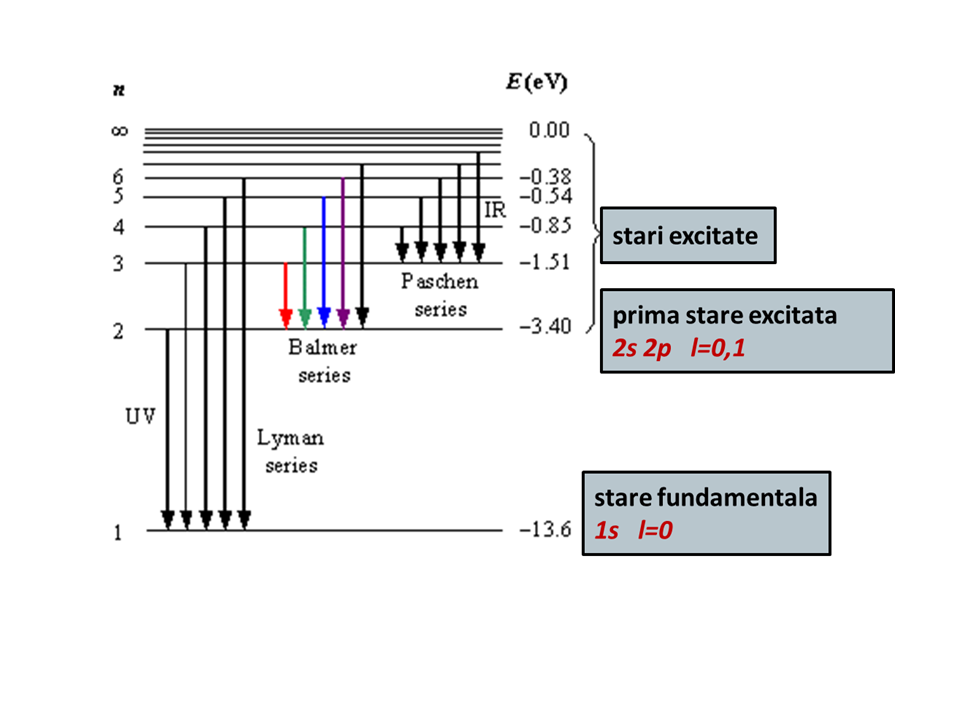
\includegraphics [width=1\textwidth]{poza-nivele-energie}
    	\caption{Nivele de energie si exemple de tranzitii intre acestea (cu spectre in domeniul UV, vizibil si IR).}
    	\label{niveleatom}
    \end{figure}
În figura \ref{niveleatom} .....